
\documentclass[twoside,11pt]{article}

\usepackage{jmlr2e}
\usepackage{hyperref}
\usepackage{amsmath}
\usepackage{soul} %for cuting line with \st{}
\usepackage{nicefrac}
\usepackage{booktabs} % for fancy tabbles
%\usepackage{amsfonts}
\usepackage[utf8]{inputenc}
\usepackage{framed}
\usepackage{color}
\usepackage{arydshln} % for dashed lines in the matrix
\newcommand*{\Scale}[2][4]{\scalebox{#1}{$#2$}}%
\jmlrheading{1}{2000}{1-48}{4/00}{10/00}{Ivo Fagundes David de Oliveira, Nir Ailon and Ori Davidov}

% Short headings should be running head and authors last names

\ShortHeadings{Supplementary Material for: A New and Flexible Approach to the Analysis of Paired Comparison Data}{Ivo Fagundes David de Oliveira, Nir Ailon and Ori Davidov}
\firstpageno{1}

\begin{document}

\title{Supplementary Material for: A New and Flexible Approach to the Analysis of Paired Comparison Data}



\author{\name Ivo F. D.\ Oliveira \email ivodavid@gmail.com \\
       \addr Department of Science, Engineering and Technology\\
       UFVJM - Federal University of the Valleys of Jequitinhonha and Mucuri\\
       Teofilo Otoni, Minas Gerais, Brazil
       \AND
       \name Nir Ailon \email nailon@cs.technion.ac.il \\
       \addr Department of Computer Science\\
       Technion - Israel Institute of Technionlogy\\
       Haifa, Israel
       \AND
       \name Ori Davidov \email davidov@stat.haifa.ac.il \\
       \addr Department of Statistics\\
       University of Haifa\\
       Haifa, Israel}

\editor{To be defined \today}


\maketitle


\section{Simulations}
In this file we reproduce experiments 1,2 and 3 and the illustrative example of Sections 5.1 and 5.2 utilizing the $\mathcal{L}_1$ and the $\mathcal{L}_{\infty}$ norms. For completeness we provide a full description of the experiments and follow up with a discussion comparing the main results for different norms. The simulations are performed 1000 times and we report the average performance under the specified conditions.

For convenience we provide a selection of results that serve as theoretical benchmarks for comparison between norms and which will help us to calibrate our expectations. The proofs are omitted for brevity. 

%\begin{proposition}%[Sensitivity Analysis: Known $F$]
%\label{the:sensitivity_LS}
%Let $F$ be a known $L$-Lipschitz continuous function with a $4U$-Lipschitz continuous inverse (over their respective domains). Let $\boldsymbol{\hat \mu} $ be the LS estimator and $\boldsymbol{P^*} = F(\Delta \boldsymbol{\hat \mu})$. Then, for the $\mathcal{L}_1$ and  $L_{\infty}$ norm we find that we find that:  \\ 
%\begin{equation}||\boldsymbol{P^*} - \boldsymbol{P}||_1  \leq 2   LU ||\boldsymbol{\hat{P}} - \boldsymbol{P} ||_1  \ \ \ \ \ \ \text{ and }  \ \ \ \ \ \ ||\boldsymbol{\hat{\mu}} - \boldsymbol{\mu} ||_1  \leq (U/n) || \boldsymbol{\hat{P}} - \boldsymbol{P}||_1;\end{equation}
%\begin{equation}|| \boldsymbol{P^*} - \boldsymbol{P}||_{\infty} \leq 2  LU ||\boldsymbol{\hat{P}} - \boldsymbol{P}||_{\infty}  \ \ \ \ \ \ \text{ and }  \ \ \ \ \ \ || \boldsymbol{\hat{\mu}} - \boldsymbol{\mu}||_{\infty} \leq U || \boldsymbol{\hat{P}} - \boldsymbol{P}||_{\infty}. \ \ \end{equation}
%\end{proposition}

\begin{proposition}%[Sensitivity Analysis - Analytic Case]
\label{the:analytic_sensitivity_LS}
Let $\boldsymbol{P^*} = F_{\boldsymbol{\hat{\beta}}}\left(\Delta \boldsymbol{\hat{\mu}}\right)$ where $\boldsymbol{\hat{\beta}}$ and $\boldsymbol{\hat{\mu}}$ are estimated with \textsc{PolyRank} using either the $\mathcal{L}_1$ or the $\mathcal{L}_{\infty}$ norm. Assume that the true probability matrix is given by  $\boldsymbol{P} = F(\Delta \boldsymbol{\mu})$ for some $\boldsymbol{\mu}$ and some unknown $L$-Lipschitz continuous function $F$ with an analytic inverse function $F^{-1}$ whose coefficients are upper-bounded by $U$. Then, if $\boldsymbol{\beta}$ and $\boldsymbol{\mu}$ were estimated using the $\mathcal{L}_1$ norm, then:
\begin{equation}
||\boldsymbol{P^*} - \boldsymbol{P}||_1\leq (1+4LU)||\boldsymbol{\hat{P}} - \boldsymbol{P}||_1  + (1/2^D)LUI^2
\end{equation}

and if $\boldsymbol{\beta}$ and $\boldsymbol{\mu}$ were estimated using the $\mathcal{L}_{\infty}$ norm, then:
\begin{equation}
||\boldsymbol{P^*} - \boldsymbol{P}||_{\infty}\leq (1+4LU)||\boldsymbol{\hat{P}} - \boldsymbol{P}||_{\infty}  + (1/2^D)LU.
\end{equation}
\end{proposition}

\begin{corollary}
Under the conditions of the above Proposition,  if $\boldsymbol{\beta}$ and $\boldsymbol{\mu}$ were estimated using the $\mathcal{L}_1$ norm, then:
\begin{equation}
||\boldsymbol{P^*} - \boldsymbol{P}||_2\leq (1+4LU)I||\boldsymbol{\hat{P}} - \boldsymbol{P}||_2  + (1/2^D)LUI^2
\end{equation}
 if $\boldsymbol{\beta}$ and $\boldsymbol{\mu}$ were estimated using the $\mathcal{L}_{\infty}$ norm, then:
\begin{equation}
||\boldsymbol{P^*} - \boldsymbol{P}||_2\leq (1+4LU)I||\boldsymbol{\hat{P}} - \boldsymbol{P}||_2  + (1/2^D)LUI.
\end{equation}
\end{corollary}

Both Proposition 1 and Corollary 2 provide sensitivity bounds analogous to those obtained for the $\mathcal{L}_2$ norm in Theorem 6 of the main text. In Proposition 1 bounds are given with respect to the corresponding norms utilized by \textsc{PolyRank}, whereas Corollary 2 gives the same bounds with with respect to the $\mathcal{L}_2$ norm. The $\mathcal{L}_2$ bounds provide a reference point to which other simulation results are compared. Notice that equations (3) and (4) of Corollary 2 show that the constant associated with the estimation error, when measured in terms of $\mathcal{L}_2$, is  $(1+4LU)I$ for both the $\mathcal{L}_1$ and the $\mathcal{L}_{\infty}$ norms, i.e., they are $I$ times bigger than the constant associated with the $\mathcal{L}_2$ norm. Also, the approximation error associated with the $\mathcal{L}_1$ norm, given by $(1/2^D)LUI^2$, is $I$ times bigger than that of the $\mathcal{L}_2$ and the $\mathcal{L}_{\infty}$ norms. Thus, we expect to see higher estimation errors than those found with the $\mathcal{L}_2$  norm and thus a slower convergence. Nevertheless, for sufficiently large $D$ and provided sufficient data, both norms are guaranteed to converge even in this agnostic setting.
\\

We proceed to the experiments.

\paragraph{Experiment 1:}  In this experiment we investigate the empirical performance of the LS refinement (given the correct comparison function) with \textsc{PolyRank} using a low degree polynomial. For this we  generate  $I = 20$ items with merits $\mu_i$ sampled uniformly from $ [0, 10]$. A total of $50$ pairs, selected randomly, were compared assuming a Bradley-Terry-Luce (BTL) model. We refine the estimator $\hat{p}_{ij} = (Y_{ij}+1)/(m_{ij}+2)$ with \textsc{PolyRank} using $D=5$. We also compute the LS estimator with known $F$.  Figures \ref{L1_figure_2},
\ref{Linf_figure_2}  show the  average distance $||\boldsymbol{P}^* - \boldsymbol{P}||_2$ of the estimator refined with the $\mathcal{L}_1$ and $\mathcal{L}_{\infty}$ norms respectively.

As expected, in both cases the LS method with the correct comparison function performs best, \textsc{PolyRank} performs almost as well and both substantially outperform the initial estimates. In this experiment, no significant difference is noticed when \textsc{PolyRank} is used with either the $\mathcal{L}_1,L_2$ or the $\mathcal{L}_{\infty}$ norms.
\begin{figure}
  \centering
    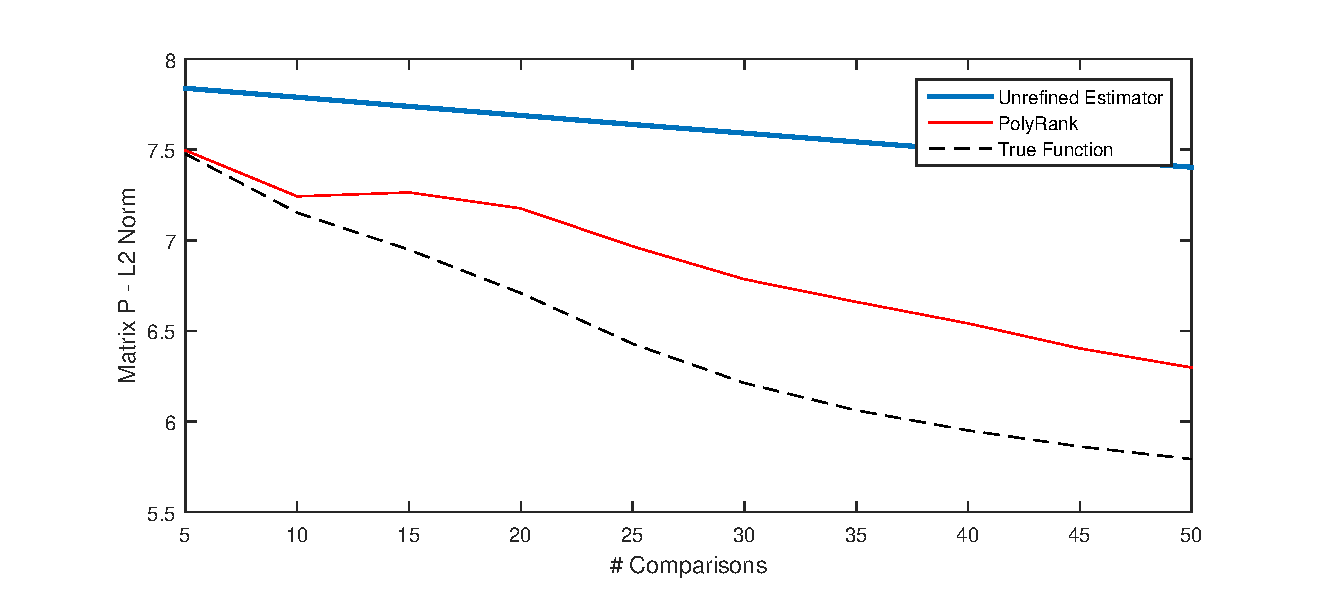
\includegraphics[width=1\textwidth]{L1_figure_2.eps}
    \caption{Comparison of estimator refined using \textsc{PolyRank} with the $\mathcal{L}_1$ norm with low sampling. \label{L1_figure_2}}
\end{figure}

\begin{figure}
  \centering
    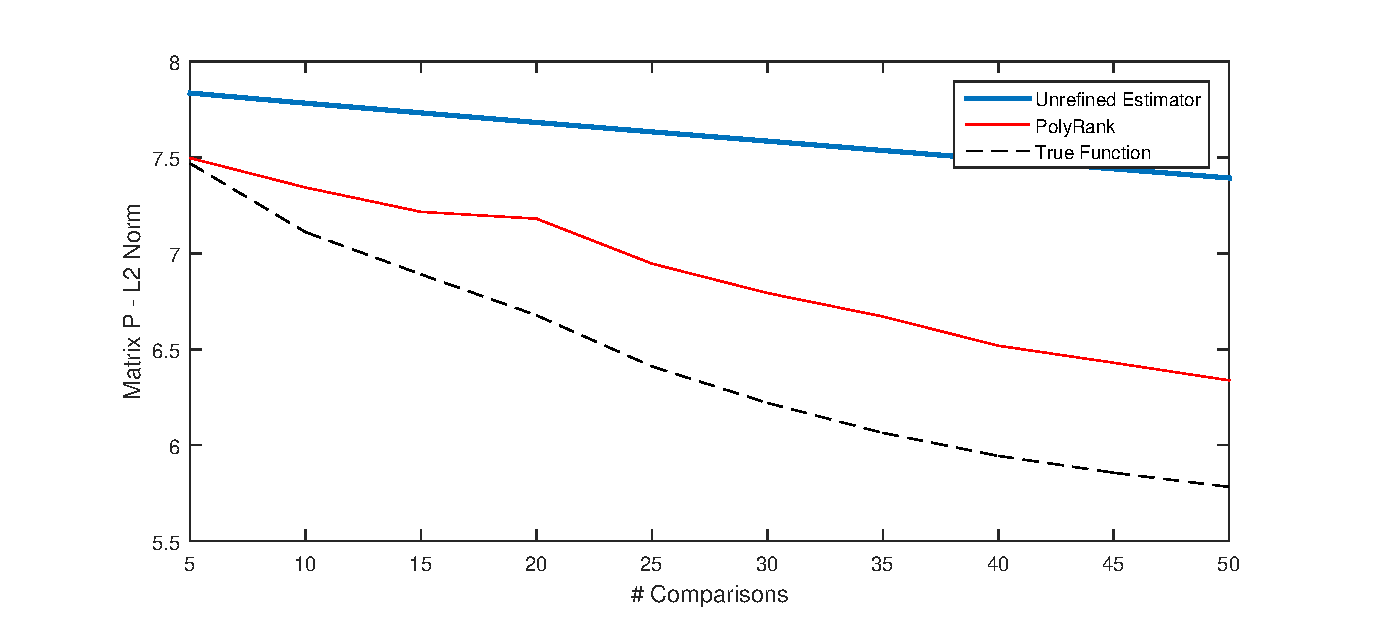
\includegraphics[width=1\textwidth]{Linf_figure_2.eps}
    \caption{Comparison of estimator refined using \textsc{PolyRank} with the $\mathcal{L}_{\infty}$ norm with low sampling. \label{Linf_figure_2}}
\end{figure}

\paragraph{Experiment 2}  In this experiment we investigate the empirical performance of  \textsc{PolyRank} in the round-robin setting with an increasing number of items. For this we generate a sequence of round-robin tournaments with  $I = 10, 20, 30, 40$ and $50$ items. The data is generated with a polynomial quantile function of degree $D=5$. The matrix $\boldsymbol{P}$ is estimated using the isotonic regression estimator of (Chatterjee, S. and  Mukherjee, S. 2016) and refined using  \textsc{PolyRank} with $D \in \{3,5,7\}$ with the $\mathcal{L}_1$ and $\mathcal{L}_{\infty}$ norms.  Figures \ref{L1_figure_3} and \ref{Linf_figure_3} display, respectively, the average of $||\boldsymbol{P}^* - \boldsymbol{P}||^2/I^2$ when the $\mathcal{L}_1$ and $\mathcal{L}_{\infty}$ norms are used in the refinement step. Figures \ref{L1_figure_4} and \ref{Linf_figure_4} display the average of $||(\boldsymbol{\hat{\beta}} -\boldsymbol{\beta}, \boldsymbol{\hat{\mu}} -\boldsymbol{\mu})||^2/(I+D)$ for the respective norms.

\begin{figure}
  \centering
    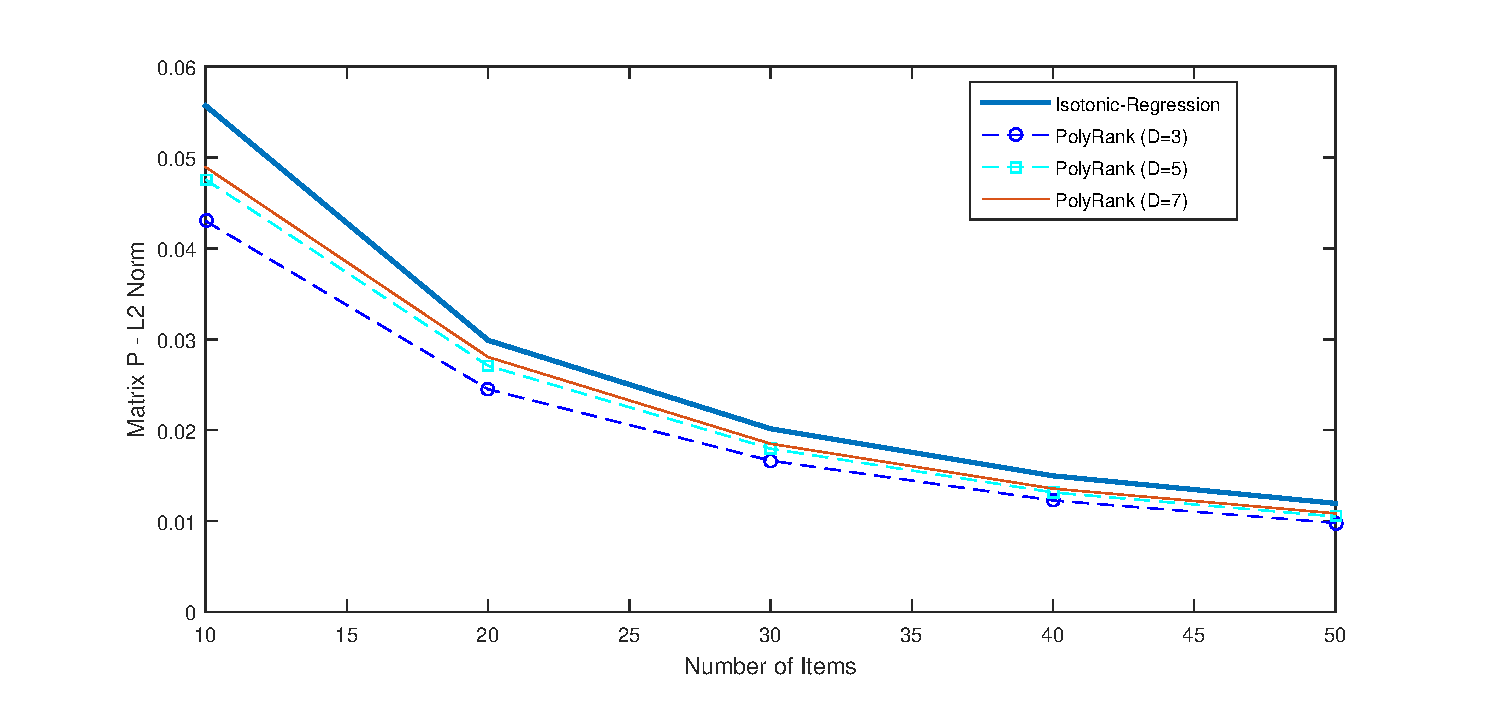
\includegraphics[width=1\textwidth]{L1_figure_3}
    \caption{Refined estimators for round-robin tournaments using the $\mathcal{L}_1$ norm. \label{L1_figure_3}}
\end{figure}

\begin{figure}
  \centering
    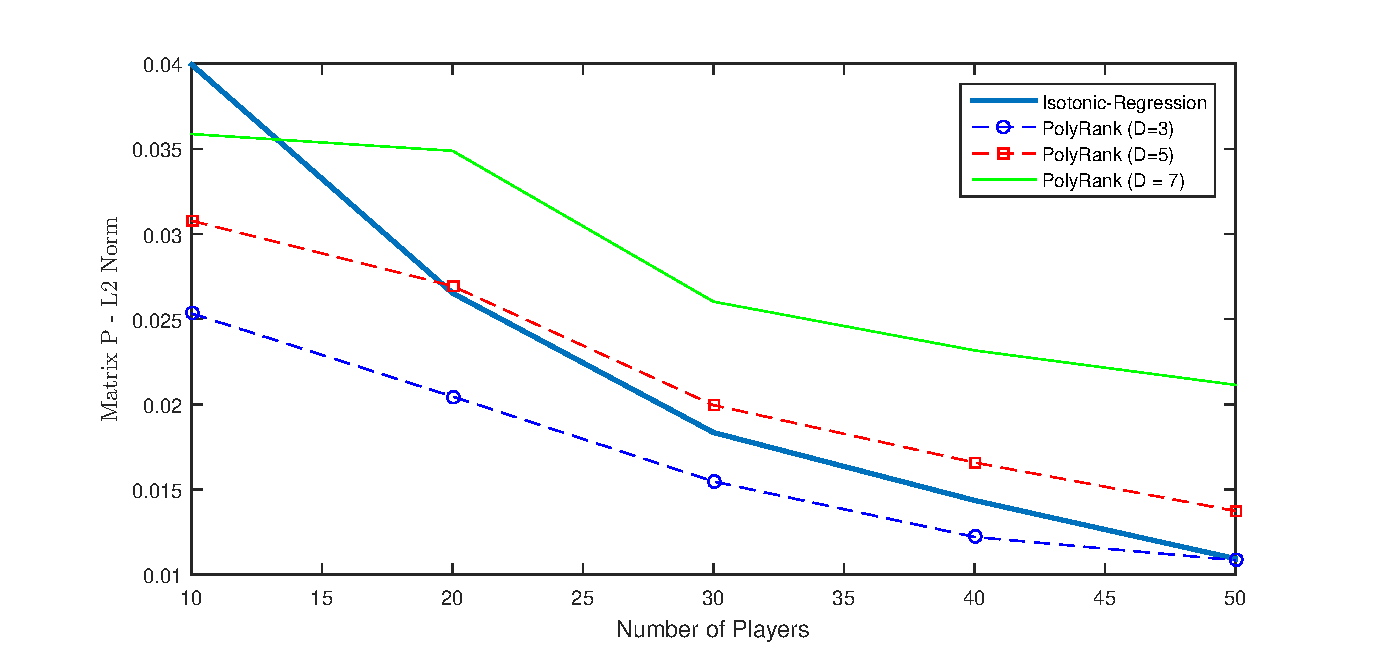
\includegraphics[width=1\textwidth]{Linf_figure_3}
    \caption{Refined estimators for round-robin tournaments using the $\mathcal{L}_{\infty}$ norm. \label{Linf_figure_3}}
\end{figure}

\begin{figure}
  \centering
    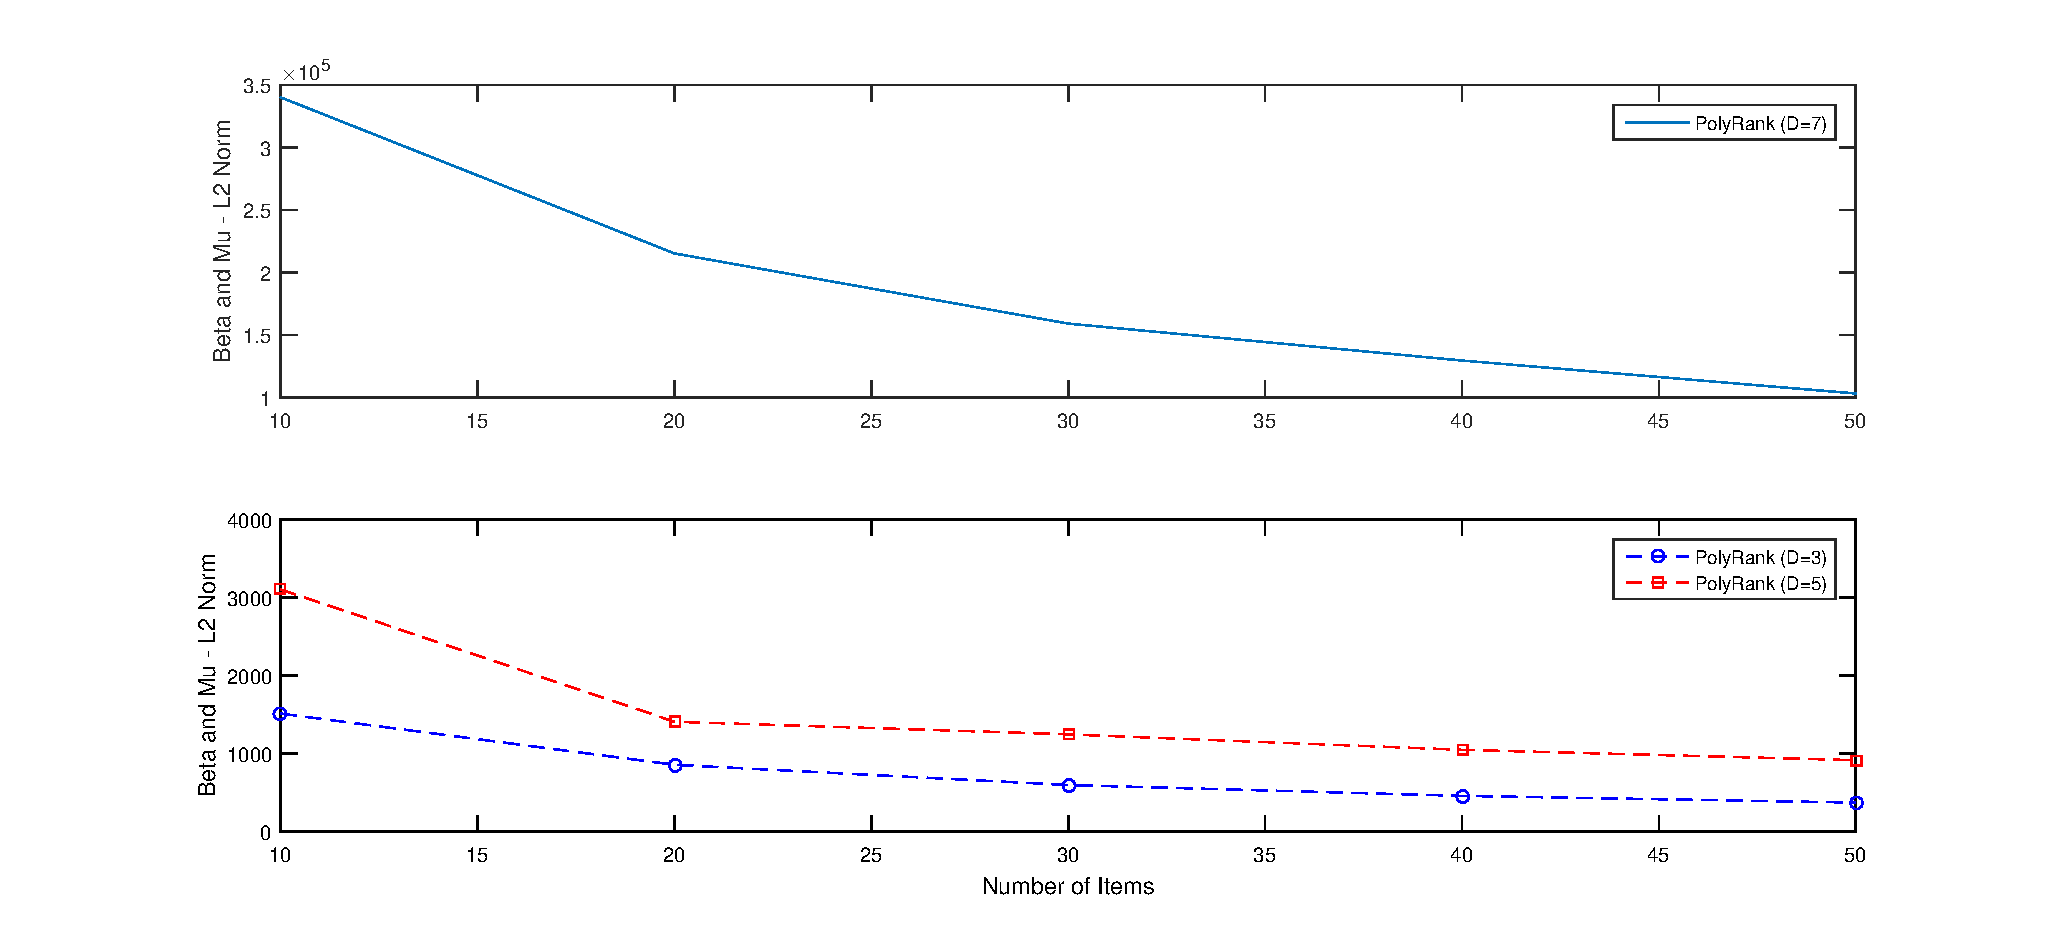
\includegraphics[width=1\textwidth]{L1_figure_4}
    \caption{Estimated parameters for round-robin tournaments using the $\mathcal{L}_1$ norm. \label{L1_figure_4}}
\end{figure}

\begin{figure}
  \centering
    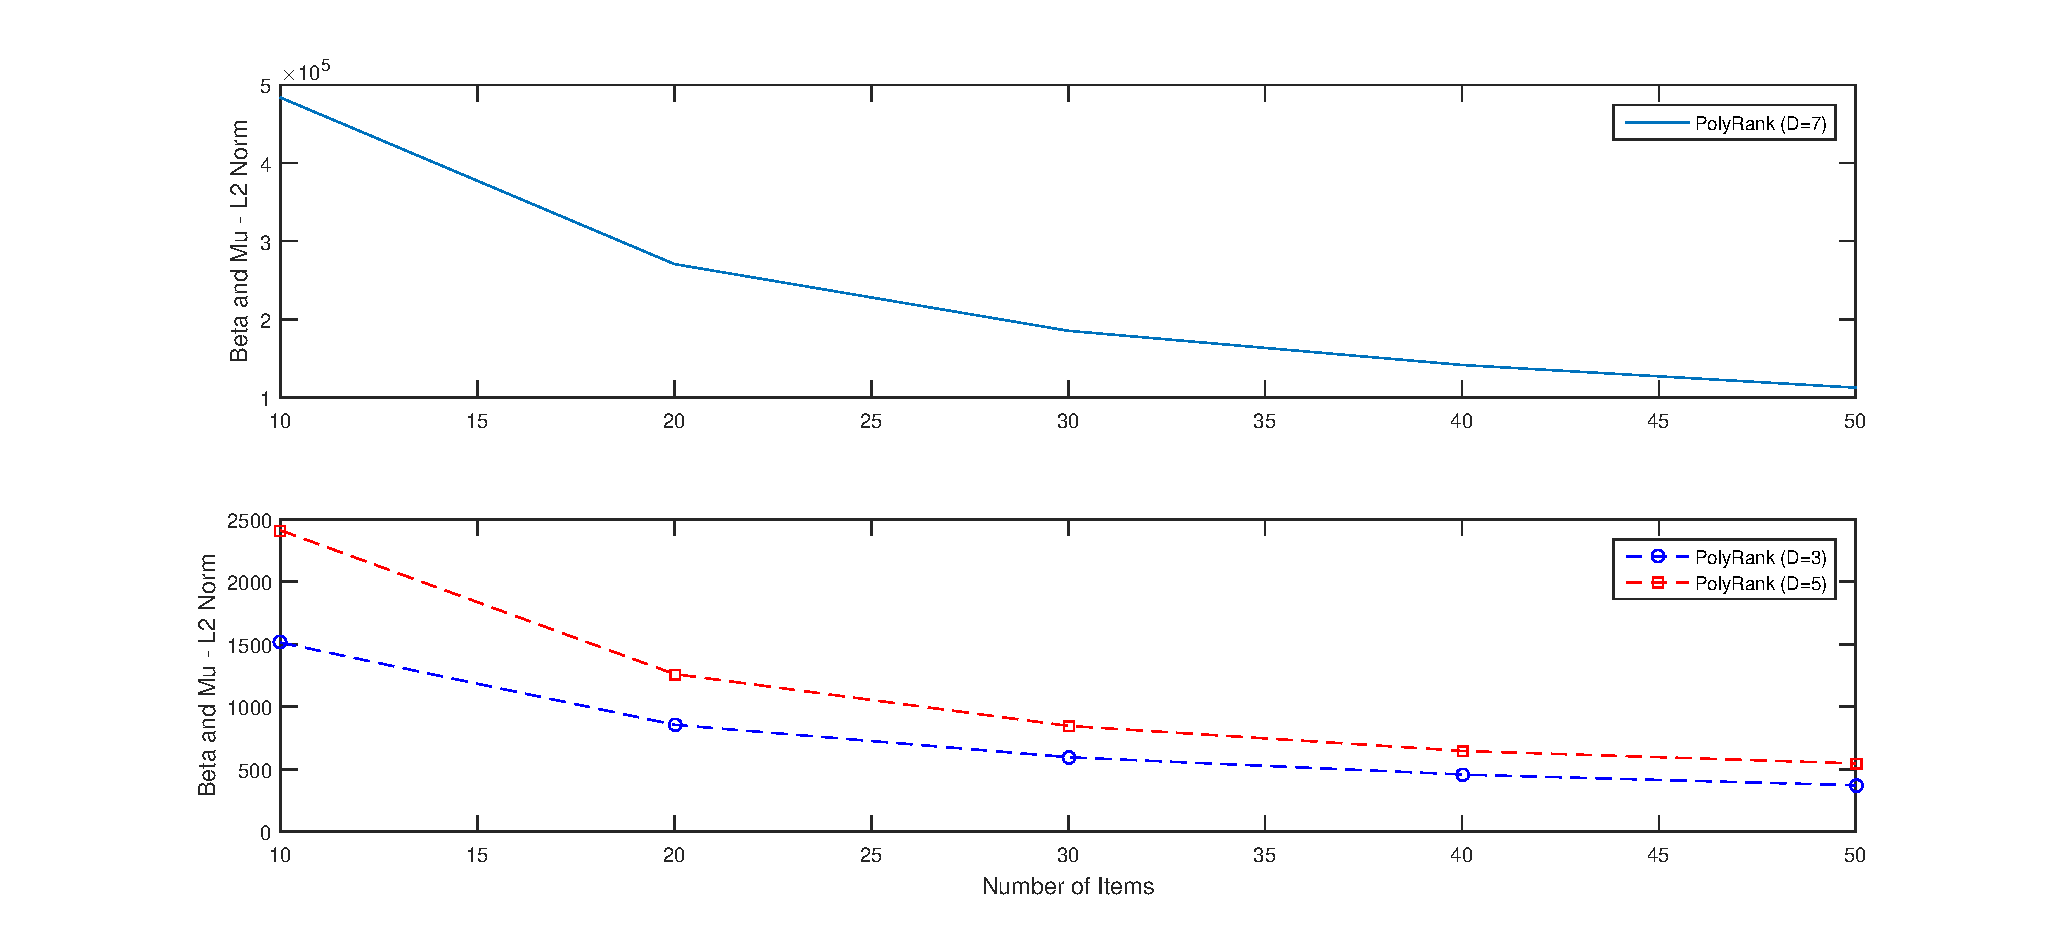
\includegraphics[width=1\textwidth]{Linf_figure_4}
    \caption{Estimated parameters for round-robin tournaments using the $\mathcal{L}_{\infty}$ norm. \label{Linf_figure_4}}
\end{figure}

Figures \ref{L1_figure_3} and \ref{Linf_figure_3} show four curves, all of which decrease with $I$. The solid blue curve is the risk for the unrefined isotonic-regression based estimator. The estimators refined by \textsc{PolyRank} correspond to the remaining curves. When the  $\mathcal{L}_1$ norm is used we find that the refined estimators always do better than the unrefined estimators. When the  $\mathcal{L}_{\infty}$ norm is used this is not the case. Even though the  $\mathcal{L}_{\infty}$ norm does not perform as well on all cases,  precision is lost at most by a constant factor in the worst case, and, in the best case we find an improvement in the overall estimator. This is consistent with our theoretical results.

Notice that in both experiments over-fitting, i.e., $D=7$, usually results in higher estimation errors  when compared to $D=3,5$ and the lowest estimation error is found when $D=3$, i.e., when under-fitting. This behavior is similar to what was found with the $\mathcal{L}_2$ norm. In Figures \ref{L1_figure_4} and \ref{Linf_figure_4} we see that the average error of the estimated parameters decreases as a function of $I$ and once again under-fitting seems to outperform the true model, and the true model outperforms overfitting.

In this experiment, no significant difference is noticed when \textsc{PolyRank} is used with either the $\mathcal{L}_1,\mathcal{L}_2$ or the $\mathcal{L}_{\infty}$ norms other than the overall speed of convergence of the estimators. When speed of convergence is critical, then, the $\mathcal{L}_2$ norms should be prefered.

\paragraph{Experiment 3:} In this experiment we investigate the empirical performance of  \textsc{PolyRank} in the round-robin setting with a fixed number of items.  For this we generate a sequence of round-robin tournaments with $I=10$ and an increasing number of matches. The data is generated using a polynomial quantile function of degree $D=3$. The matrix $\boldsymbol{P}$ is estimated using the standard frequency estimator for $\hat{p}_{ij} $   and is refined using  \textsc{PolyRank} (with $D=3$). Figures \ref{L1_figure_5} and \ref{Linf_figure_5} display the average of $||\boldsymbol{P}^* - \boldsymbol{P}||^2/I^2$, of $||\boldsymbol{\hat \mu} - \boldsymbol{\mu}||^2/I$ and of $||\boldsymbol{\hat \beta} - \boldsymbol{\beta}||^2$ for $m_{ij}  = 1, 3, 5, 7$ and $9$ for all pairs $(i,j)$ when the $\mathcal{L}_1$ and the $\mathcal{L}_{\infty}$ norms are used in the refinement step. Figures \ref{L1_figure_6} and \ref{Linf_figure_6} show the sequence of estimated functions when the $\mathcal{L}_1$ and the $\mathcal{L}_{\infty}$ norms are used in the refinement step.

For both norms we observe a similar behavior. The top two curves of Figures \ref{L1_figure_5} and \ref{Linf_figure_5} show that the variance of the estimators $\boldsymbol{P}^*$ and  $\hat{\boldsymbol{\mu}}$ decreases with the amount of paired comparisons in both experiments. The bottom curves of Figures \ref{L1_figure_5} and \ref{Linf_figure_5} show the variance of the estimator $\hat{\boldsymbol{\beta}}$, and, in both cases the estimator did not converge. Figures \ref{L1_figure_6} and \ref{Linf_figure_6} show that the graph of the estimated comparison functions do not match the true function due to the slow convergence. 

\begin{figure}
  \centering
    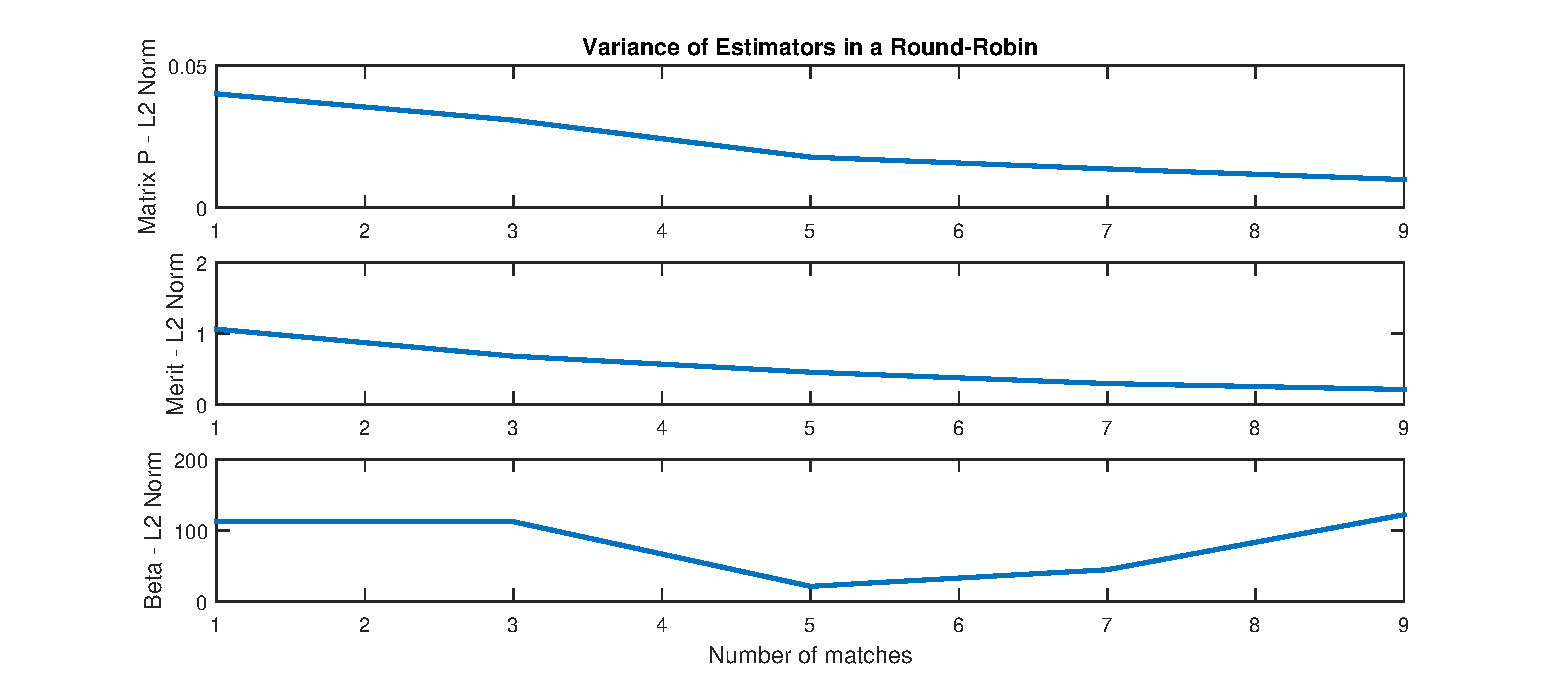
\includegraphics[width=1\textwidth]{L1_figure_5}
    \caption{Variance of estimators in a round-robin with increasing number of matches between each pair using the $\mathcal{L}_1$ norm. \label{L1_figure_5}}
\end{figure}

\begin{figure}
  \centering
    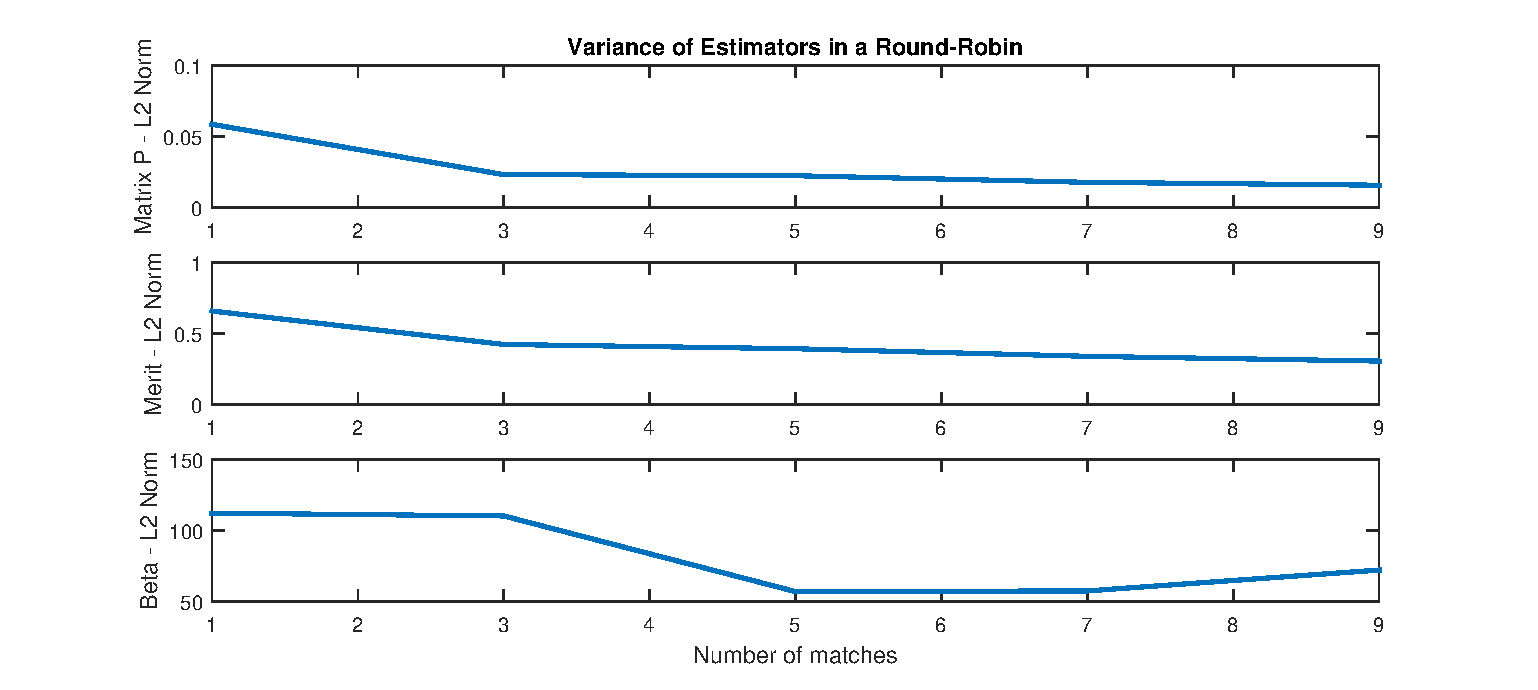
\includegraphics[width=1\textwidth]{Linf_figure_5}
    \caption{Variance of estimators in a round-robin with increasing number of matches between each pair using the $\mathcal{L}_{\infty}$ norm. \label{Linf_figure_5}}
\end{figure}

\begin{figure}
  \centering
    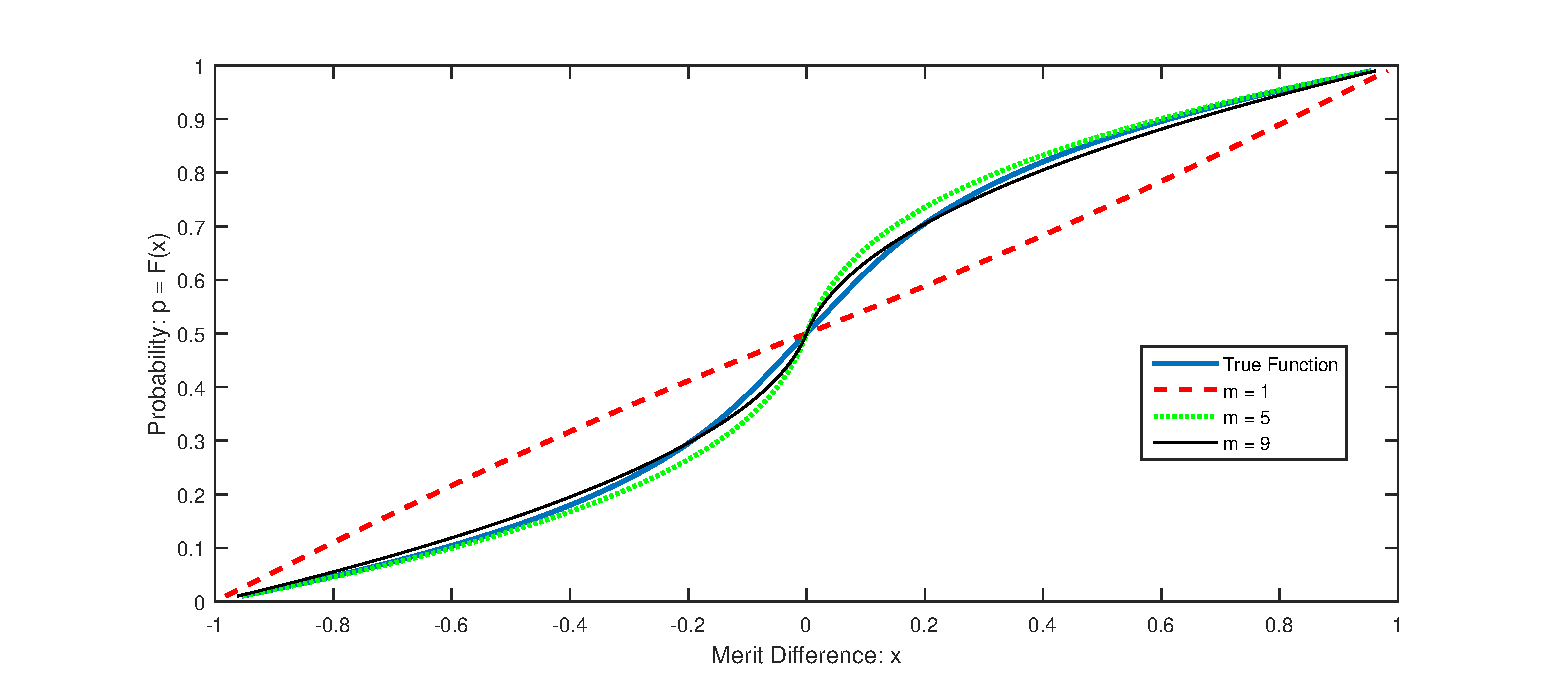
\includegraphics[width=1\textwidth]{L1_figure_6}
    \caption{Recovered function using the $\mathcal{L}_1$ norm. \label{L1_figure_6}}
\end{figure}

\begin{figure}
  \centering
    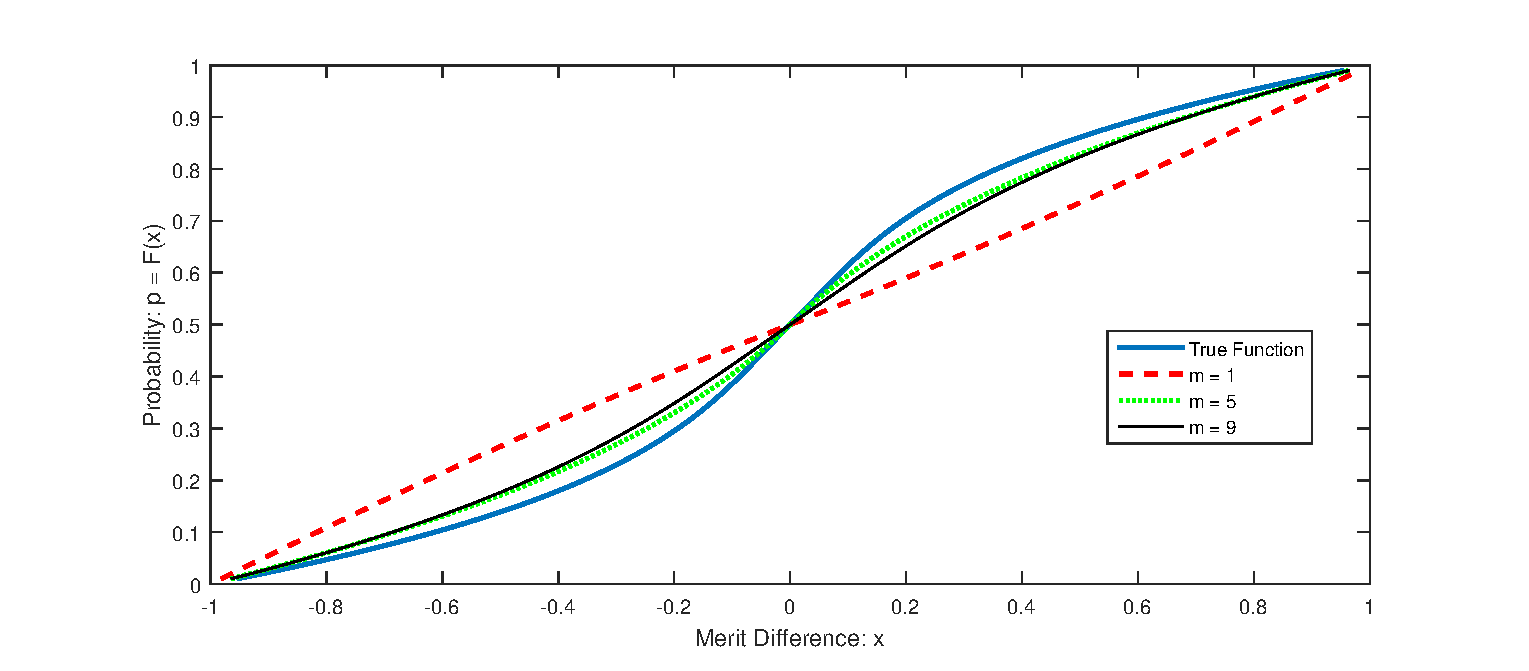
\includegraphics[width=1\textwidth]{Linf_figure_6}
    \caption{Recovered function  using the $\mathcal{L}_{\infty}$ norm. \label{Linf_figure_6}}
\end{figure}



\subsection{Illustrative Example}

In this subsection we illustrate the use of \textsc{PolyRank} on a computer-chess dataset\footnote{Publicly available at \url{http://kirill-kryukov.com/chess/kcec/games.html}.}. The dataset comprises of matches between $186$ free single-CPU chess-engines. Each chess-engine played (roughly) $32$ matches against $40$  opponents. We use \textsc{PolyRank} to estimate model parameters from observed matches that resulted in a victory or defeat; ties are ignored. Figures \ref{L1_figure_7} and \ref{Linf_figure_7} show the estimated comparison function for various values of $D$ for the first 100 chess-engines using \textsc{PolyRank} with the $\mathcal{L}_1$ and the $\mathcal{L}_{\infty}$ norms.

In this experiment the comparison function found by \textsc{PolyRank}
utilizing both the $\mathcal{L}_1$ and the $\mathcal{L}_2$ norms are very similar, whereas the $\mathcal{L}_{\infty}$ norm differs considerably. For both norms, the function considered seems to stabilize for  $D$ greater than or equal to $7$. Figures \ref{L1_figure_8} and \ref{Linf_figure_8} show the estimated function when the dimension $D = 7$ is fixed and the number of chess-engines $I$ is gradually increased for the $\mathcal{L}_1$ and the $\mathcal{L}_{\infty}$ refined estimators. For $I$ greater than or equal to $60$ the estimated functions also seem to stabilize. Finally, Figures \ref{L1_figure_9} and \ref{Linf_figure_9} compare the best fit functions recovered by \textsc{PolyRank} to the family of BTL models described by $F_{\text{BTL}}(x) = 1/(1+\exp(-\kappa x))$ for various values of $\kappa >0$. Again, the $\mathcal{L}_1$ norm seems to recover the same function as the $\mathcal{L}_2$ norm, which, as observed in the main paper considerably differs from the BTL models. The $\mathcal{L}_{\infty}$ norm, however, seem to not have converged, perhaps because in these experiments, the expected value of $||\hat{\boldsymbol{P}}- \boldsymbol{P}||_{\infty}$ grows with the increasing number of items when the number of matches remains fixed.

\begin{figure}
  \centering
    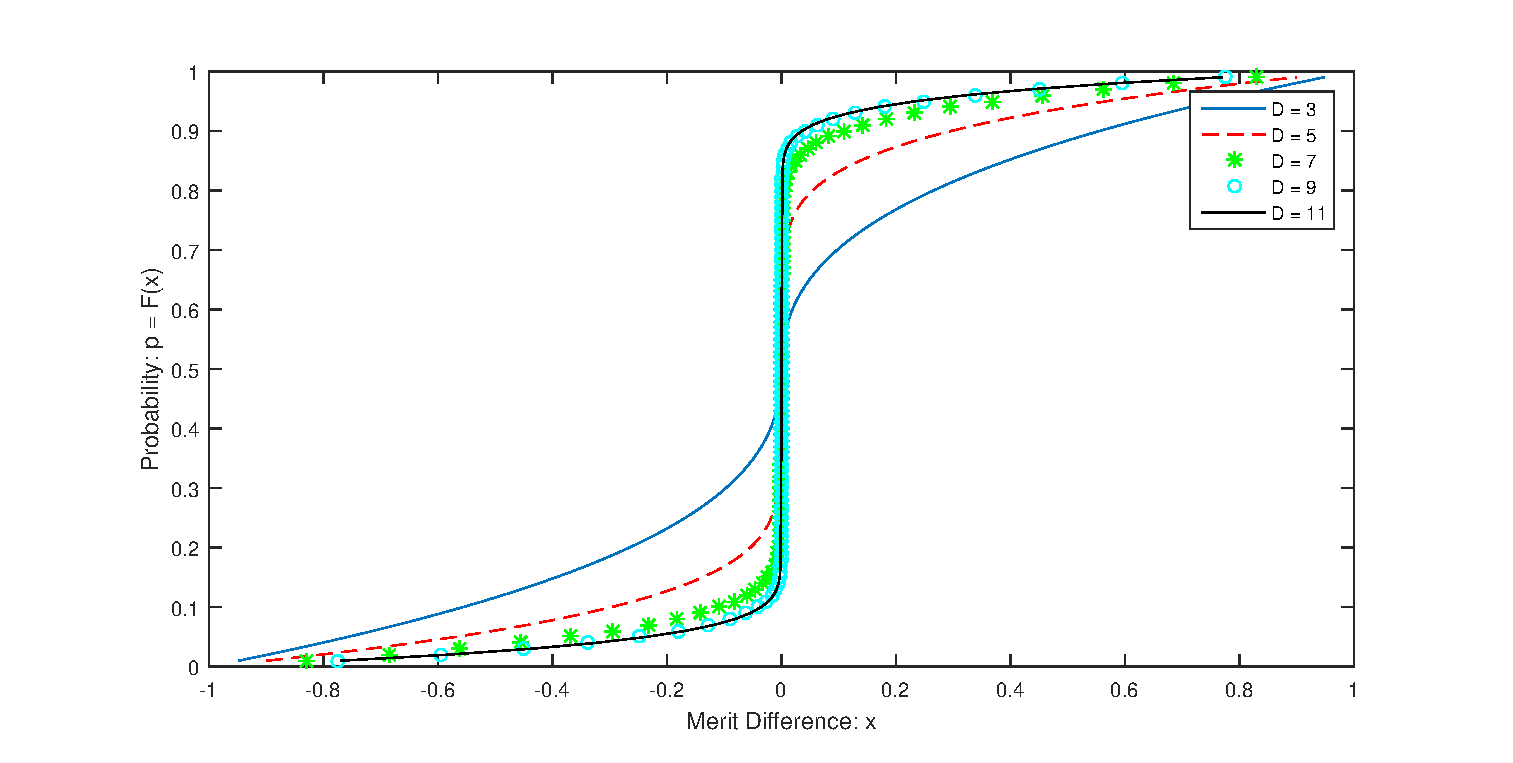
\includegraphics[width=1\textwidth]{L1_figure_7}
    \caption{The effect of increasing the dimension $D$ in estimating function $F$ obtained with the $\mathcal{L}_{1}$ norm. \label{L1_figure_7}}
\end{figure}

\begin{figure}
  \centering
    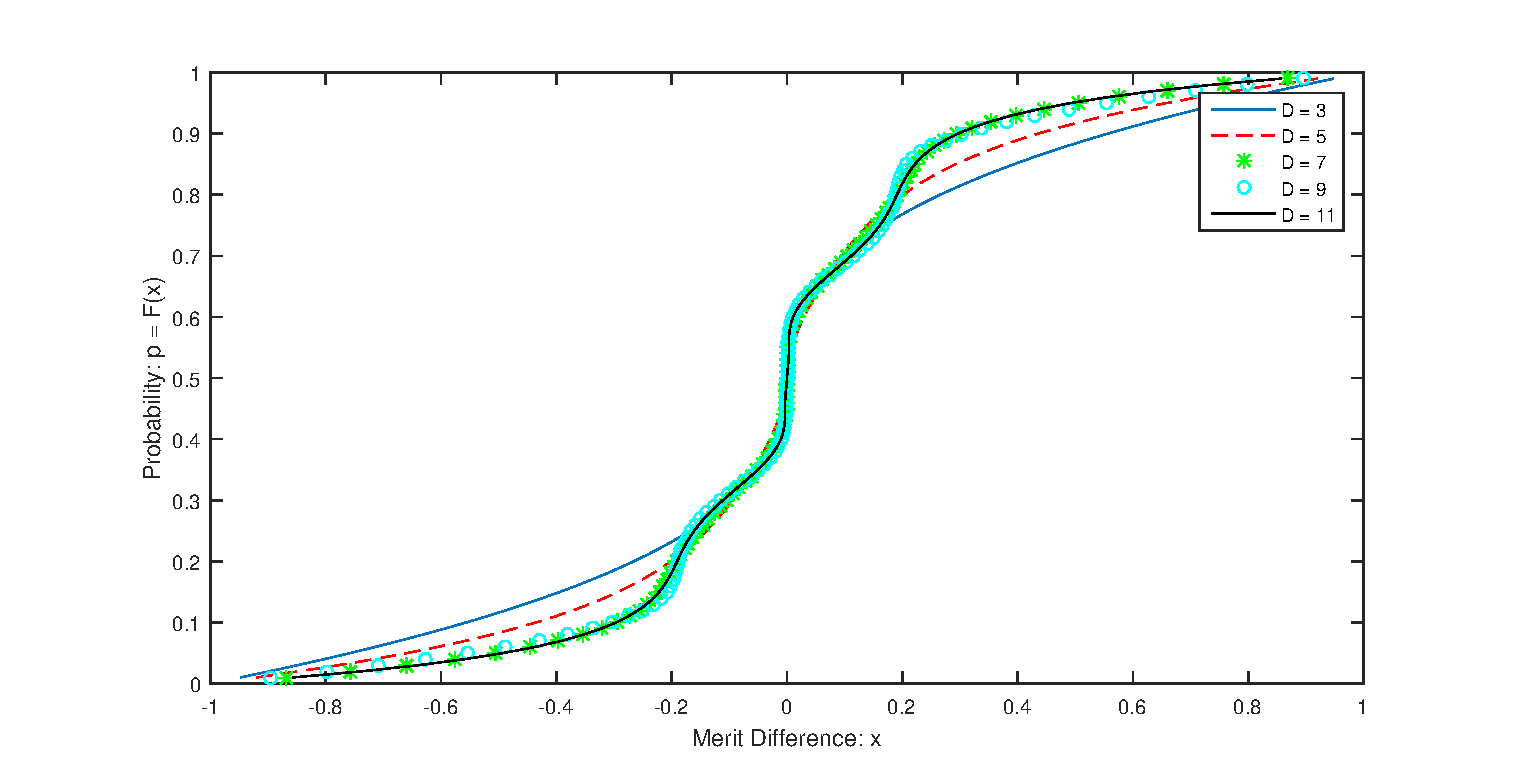
\includegraphics[width=1\textwidth]{Linf_figure_7}
    \caption{The effect of increasing the dimension $D$ in estimating function $F$ obtained with the $\mathcal{L}_{\infty}$ norm. \label{Linf_figure_7}}
\end{figure}

\begin{figure}
  \centering
    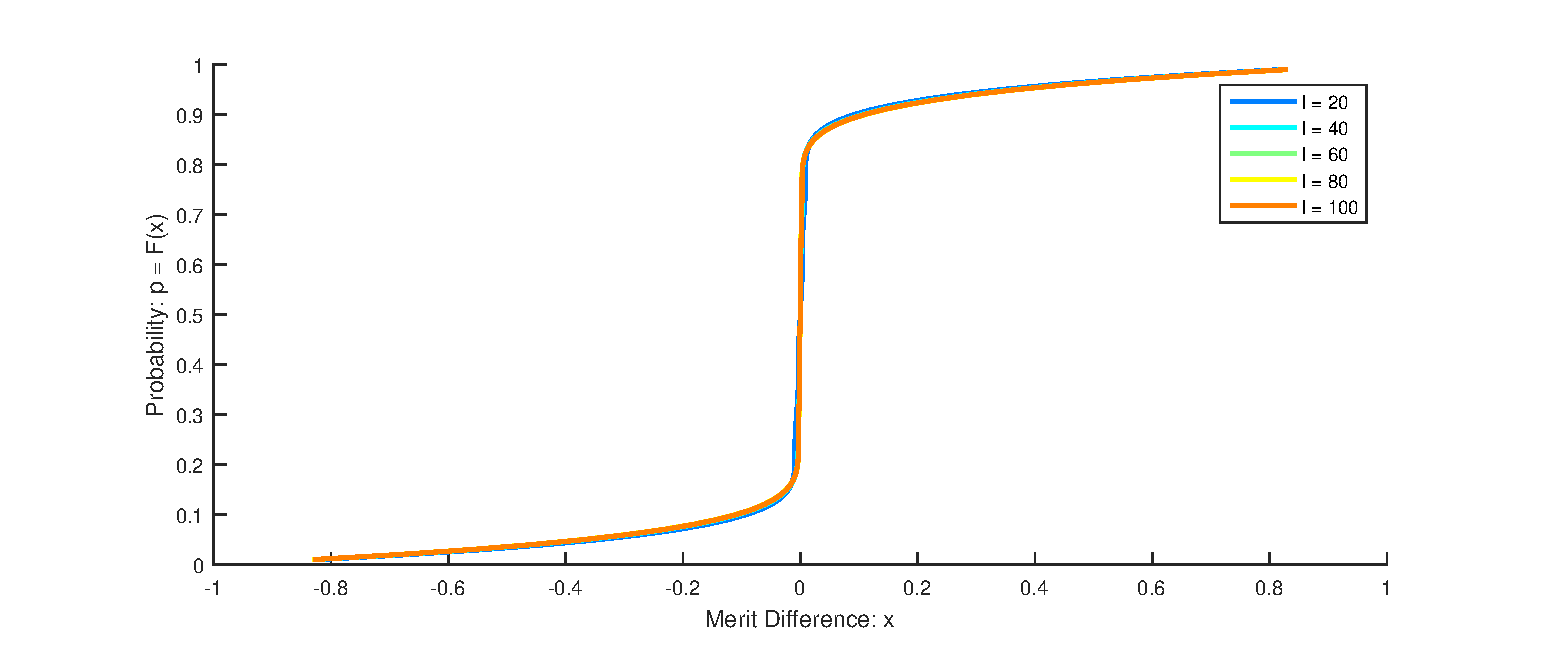
\includegraphics[width=1\textwidth]{L1_figure_8}
    \caption{The effect of increasing the amount of data in estimating function $F$ obtained with the $\mathcal{L}_{1}$ norm. \label{L1_figure_8}}
\end{figure}

\begin{figure}
  \centering
    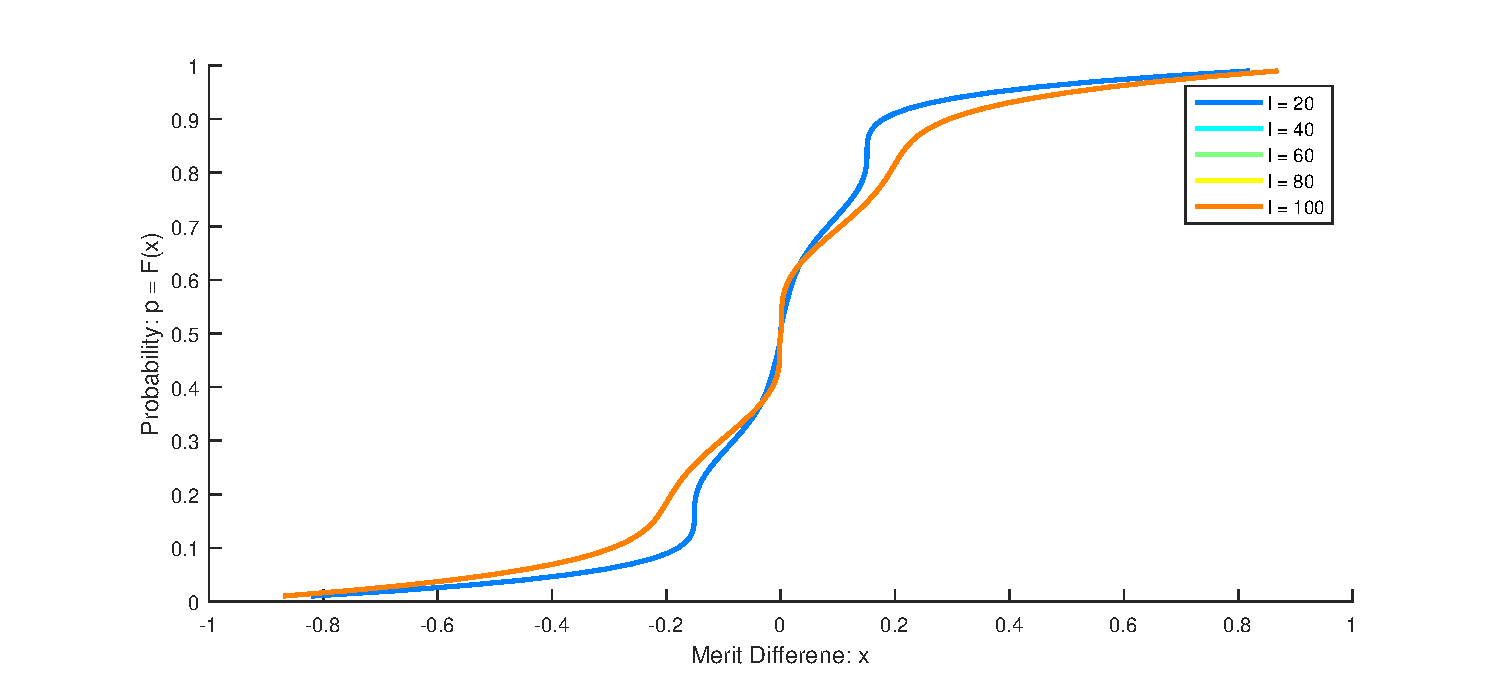
\includegraphics[width=1\textwidth]{Linf_figure_8}
    \caption{The effect of increasing the amount of data in estimating function $F$ obtained with the $\mathcal{L}_{\infty}$ norm. \label{Linf_figure_8}}
\end{figure}

\begin{figure}
  \centering
    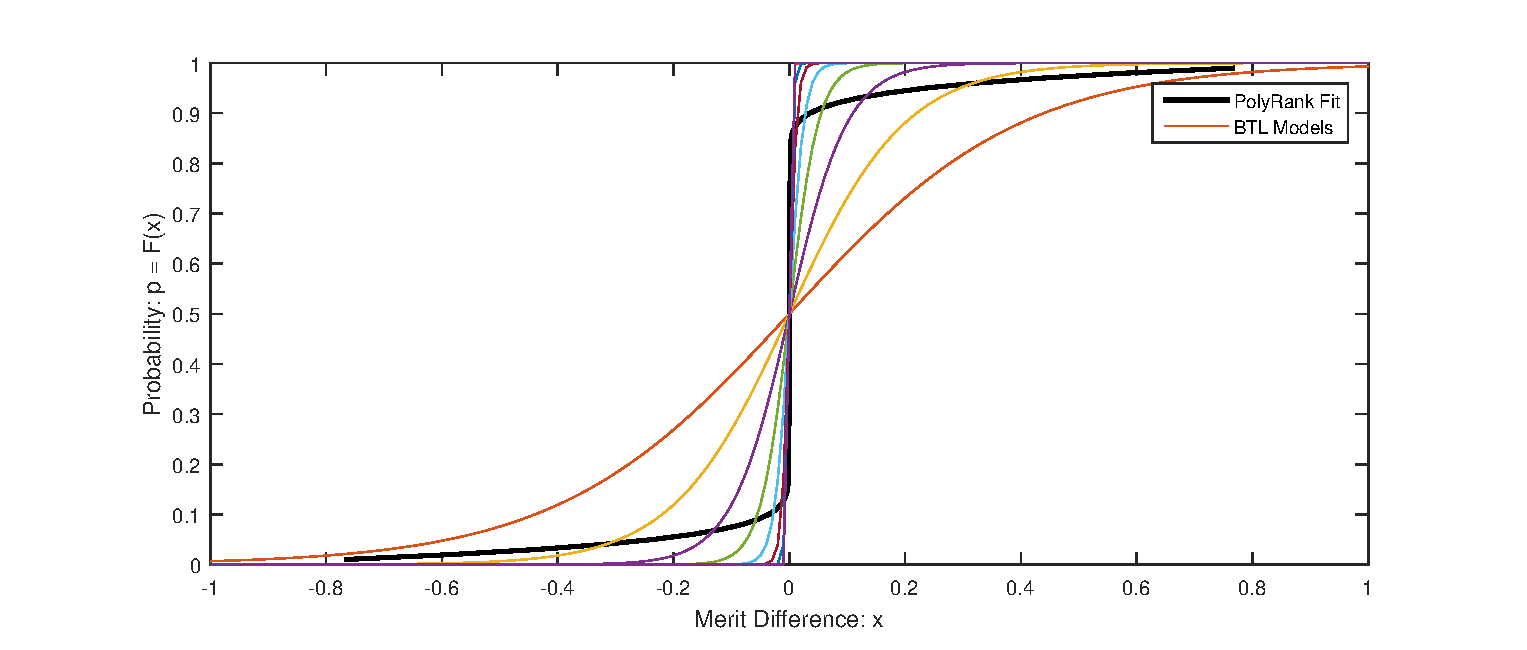
\includegraphics[width=1\textwidth]{L1_figure_9}
    \caption{Bradley-Terry-Luce models compared to the best fit comparison function obtained with the $\mathcal{L}_{1}$ norm. \label{L1_figure_9}}
\end{figure}

\begin{figure}
  \centering
    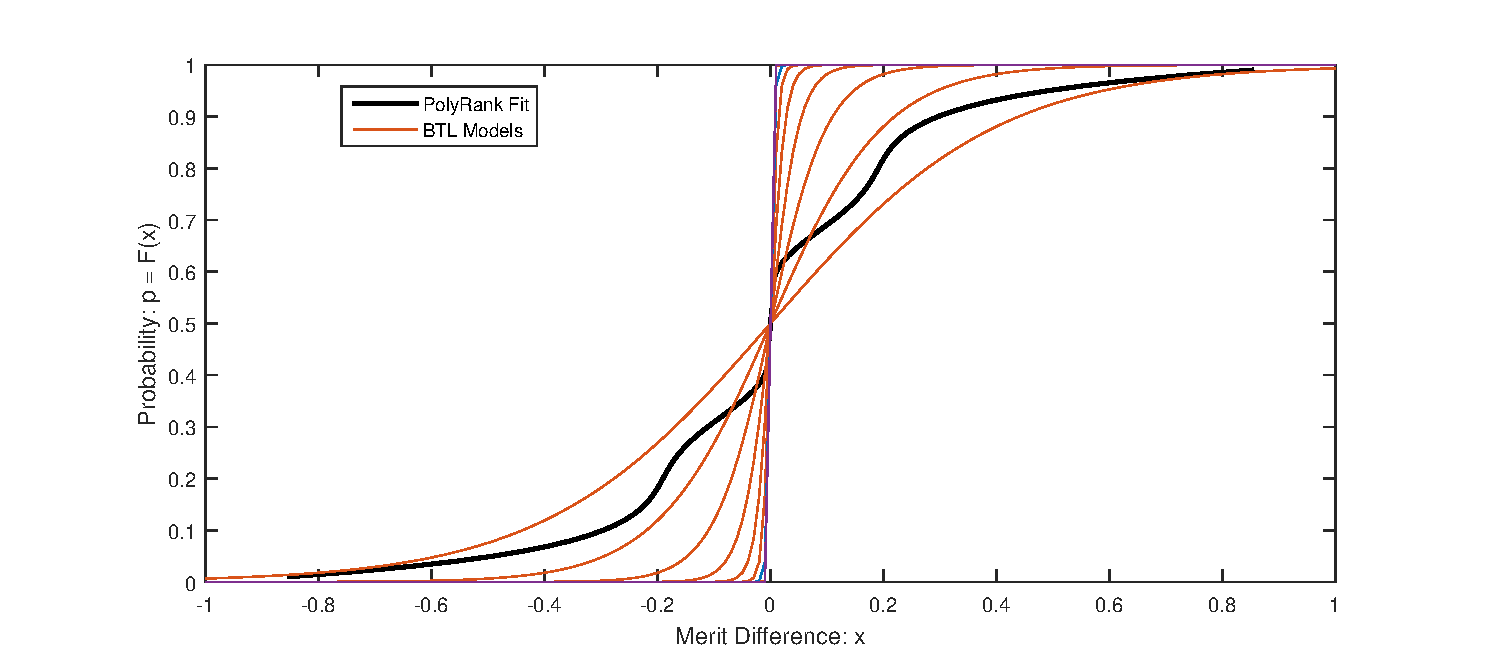
\includegraphics[width=1\textwidth]{Linf_figure_9}
    \caption{Bradley-Terry-Luce models compared to the best fit comparison function obtained with the $\mathcal{L}_{\infty}$ norm. \label{Linf_figure_9}}
\end{figure}

\subsection{Concluding Remarks}

We observe that the $\mathcal{L}_{\infty}$ norm seems to converge slower than the $\mathcal{L}_{1}$ and $\mathcal{L}_{2}$ norms. At times the $\mathcal{L}_{\infty}$ even performs worse than the unrefined estimators. The  $\mathcal{L}_{2}$ norm seems to slightly outperform the $\mathcal{L}_{1}$ norm in most experiments, though from a practitioner's perspective, the both the $\mathcal{L}_{2}$ and the the $\mathcal{L}_{1}$ norms can be chosen. As a rule of thumb, if performance is measured in terms of variance of the estimators, then, we recommend the $\mathcal{L}_2$ norm minimization. 

\end{document}